% =============================================================================
%  Chapitre 3 — Architecture : la chaîne de données et les garde-fous
%
%  Chapitre d'ingénierie, écrit dans le même registre accessible que le
%  chapitre 2 : ce que fait chaque brique, pourquoi elle existe, et quelle
%  erreur elle rend impossible. Les captures d'écran (Dagster, MLflow) et la
%  figure du pipeline DVC sont produites à partir du dépôt lui-même.
% =============================================================================

\chapter{Architecture : la chaîne de données et les garde-fous}
\label{chap:architecture}

\section*{Ce que ce chapitre explique}
\addcontentsline{toc}{section}{Ce que ce chapitre explique}

Le chapitre~\ref{chap:problematique} a posé quatre échecs à corriger. Celui-ci
décrit la machine construite pour y répondre — non pas les modèles eux-mêmes,
qui font l'objet du chapitre suivant, mais la chaîne qui les alimente et le
dispositif qui les surveille.

Le fil conducteur tient en une phrase, et c'est la décision d'ingénierie la plus
structurante du projet~: \textbf{une règle importante n'est pas documentée, elle
est rendue exécutable}. Interdire à un modèle de consulter le futur, garantir que
deux documents citent le même chiffre, imposer que chaque fonction déclare le
problème qu'elle traite — chacune de ces règles est, dans ce dépôt, un test qui
échoue si on la viole. La raison est empirique~: les trois incidents les plus
coûteux du projet, relatés en fin de chapitre, ont tous consisté en une règle
respectée par discipline jusqu'au jour où elle ne l'a plus été, sans que rien ne
le signale.

% =============================================================================
\section{Trois couches, une seule direction}
% =============================================================================

Les données brutes d'un marché financier sont hétérogènes~: des cours d'actions
marocaines relevés à la Bourse de Casablanca, des cours de fonds indiciels
américains, des indicateurs macroéconomiques publiés par la Réserve fédérale
américaine et par Bank Al-Maghrib. Chaque source a son calendrier, son format,
ses trous et ses erreurs. Les mélanger sans discipline produit un jeu de données
dont plus personne ne sait comment il a été fabriqué.

\begin{definitionbox}{Architecture en médaillon}
Organisation d'un entrepôt de données en couches successives, chacune obtenue par
transformation \emph{déterministe} de la précédente~: \textbf{Bronze} (les données
telles que reçues, jamais modifiées), \textbf{Silver} (les mêmes données
alignées, nettoyées et validées), \textbf{Gold} (les tableaux directement
exploitables par un modèle). Une couche ne lit jamais une couche située en aval
d'elle~; l'information ne circule que dans un sens.
\end{definitionbox}

Ce projet applique ce patron strictement (tableau~\ref{tab:couches}). Son intérêt
n'est pas esthétique~: il rend chaque anomalie \emph{localisable}. Si un chiffre
final surprend, il existe exactement une couche où l'erreur a pu naître, et les
couches amont sont intactes pour le prouver.

\begin{table}[htbp]
  \centering
  \small
  \caption[Les trois couches de données]{Les trois couches de données, leur
  contenu et la garantie que chacune apporte.}
  \label{tab:couches}
  \begin{tabular}{@{}p{2.1cm}p{5.1cm}p{5.4cm}@{}}
    \toprule
    \textbf{Couche} & \textbf{Contenu} & \textbf{Garantie apportée} \\
    \midrule
    Bronze &
    Cours ETF, cours et dividendes BVC, indicateurs macro, taux de change — au
    format reçu. &
    Immuable. Une source qui change produit un nouveau fichier, jamais une
    réécriture~: l'historique reste auditable. \\
    \addlinespace
    Silver &
    Rendements logarithmiques, calendriers alignés (la Bourse de Casablanca et
    les places américaines ne ferment pas les mêmes jours), zones d'illiquidité
    signalées. &
    Validée à l'écriture par un contrat de données~: rendement journalier borné à
    $\pm 50$~\%, au moins 500~lignes, index trié, aucune valeur manquante. Une
    violation interrompt le traitement. \\
    \addlinespace
    Gold &
    Deux matrices de rendements (une par univers), variables ML causales, tests
    de stationnarité, résultats des comparaisons de stratégies. &
    Seule couche que la modélisation a le droit de lire. Aucun modèle n'ouvre un
    fichier Bronze ou Silver. \\
    \bottomrule
  \end{tabular}
\end{table}

Deux conventions méritent d'être signalées, parce qu'elles paraissent techniques
et sont en réalité des décisions de fond.

\textbf{Les rendements sont logarithmiques}, c'est-à-dire calculés comme
$\ln(P_t/P_{t-1})$ plutôt que comme la variation en pourcentage. La raison est
qu'ils s'additionnent~: le rendement d'une semaine est la somme des cinq
rendements quotidiens, ce qui n'est pas vrai des pourcentages. Toute la chaîne en
dépend.

\textbf{Les trous de calendrier sont comblés vers l'avant, jamais vers
l'arrière.} Si la Bourse de Casablanca est fermée un jour où New York est
ouverte, on reporte le dernier cours \emph{connu}. Combler avec le cours
\emph{suivant} — techniquement plus simple, et proposé par toutes les
bibliothèques — reviendrait à injecter dans le passé une information du futur.
C'est la première forme, et la plus discrète, du biais que le chapitre~2 a
appelé P4.

% =============================================================================
\section{Deux univers, et un manque assumé}
% =============================================================================

Le portefeuille visé par EURAFRIC mêle quatre valeurs de la Bourse de Casablanca
— Maroc Telecom, Attijariwafa Bank, CIH Bank, Banque Centrale Populaire — et cinq
fonds indiciels internationaux couvrant les grandes actions américaines, les
technologiques, les marchés émergents, l'or et les obligations d'État.

Un obstacle est apparu dès la première semaine~: \textbf{aucune source gratuite ne
fournit l'historique de la Bourse de Casablanca avant la mi-2021}. Le portefeuille
complet ne peut donc pas être étudié sur le krach de 2020, ni sur la crise de
2008. Plutôt que de dissimuler cette limite ou d'acheter un historique, nous
avons adopté une \textbf{double base de test} (tableau~\ref{tab:univers})~: toute
stratégie est évaluée sur les deux univers, et les deux résultats sont publiés
côte à côte.

\begin{table}[htbp]
  \centering
  \small
  \caption[Les deux univers de test]{Les deux univers d'évaluation. Toute
  stratégie du projet est exécutée sur les deux, sans exception.}
  \label{tab:univers}
  \begin{tabular}{@{}lrrl@{}}
    \toprule
    \textbf{Univers} & \textbf{Actifs} & \textbf{Jours} & \textbf{Période et intérêt} \\
    \midrule
    \texttt{full\_2021} & 9 & 1\,321 &
    2021-07 $\rightarrow$ 2026-07 — le portefeuille réel visé \\
    \texttt{etf\_2017} & 5 & 5\,656 &
    2004-11 $\rightarrow$ 2026-07 — inclut 2008, 2020 et 2022 \\
    \bottomrule
  \end{tabular}
\end{table}

Ce choix a un coût de rédaction — il faut commenter deux résultats au lieu d'un,
et ils ne concordent pas toujours — mais il a une vertu décisive~: une conclusion
qui ne tient que sur un seul univers se voit immédiatement. Le
chapitre~\ref{chap:resultats} montre que c'est précisément le cas du résultat
principal.

\begin{remarquebox}
L'univers ETF a été étendu de 2017 à 2004 en cours de projet, lorsque nous avons
constaté que la date de départ initiale était une décision arbitraire et non une
limite des données. Les douze années supplémentaires ont réduit la largeur des
intervalles de confiance d'environ 38~\% et ajouté la crise de 2008. Le nom
technique de l'univers, \texttt{etf\_2017}, est resté~: le renommer aurait
invalidé les artefacts déjà produits, pour un gain purement cosmétique.
\end{remarquebox}

% =============================================================================
\section{Le dividende manquant : un défaut trouvé tardivement}
% =============================================================================

Cet épisode est rapporté en détail parce qu'il illustre mieux que tout autre le
type de défaut contre lequel l'architecture doit protéger~: silencieux, non
détecté par les tests existants, et \emph{favorable} au résultat que nous
espérions.

\begin{definitionbox}{Dividende}
Part du bénéfice qu'une entreprise verse à ses actionnaires, généralement une
fois par an. Un actionnaire gagne donc de deux manières~: la hausse du cours, et
les dividendes encaissés. Ne compter que la première revient à sous-estimer
durablement ce que l'actif a réellement rapporté.
\end{definitionbox}

La chaîne mélangeait deux définitions du rendement sans que personne ne l'ait
décidé. Les cours des fonds indiciels arrivaient \emph{ajustés des dividendes}
(rendement total), tandis que les cours de la Bourse de Casablanca arrivaient
\emph{hors dividendes}. Les rendements du dividende publiés pour ces quatre
valeurs s'échelonnent de 3,8~\% à 5,5~\% par an~: c'est l'ordre de grandeur de la
performance qui disparaissait chaque année du côté marocain.

L'instinct veut qu'un biais commun s'annule dans une comparaison. \textbf{Il ne
s'annule pas ici}, et la raison est instructive. La stratégie équipondérée est
\emph{contrainte} de détenir les actifs sous-évalués~; les optimiseurs sont
\emph{libres} de les sous-pondérer — et ils l'ont fait, précisément parce que le
dividende manquant les faisait paraître moins bons qu'ils ne l'étaient. Les
modèles étaient donc crédités d'avoir évité un défaut de notre propre traitement
de données. Le biais gonflait mécaniquement l'avantage mesuré du ML.

La correction a nécessité d'écrire un collecteur dédié~: l'interface publique
prévue à cet effet dans la bibliothèque utilisée était hors service, et les
montants ont dû être extraits du site de la Bourse de Casablanca, \emph{avec leur
date de détachement} — car un dividende doit être crédité le jour où il est
effectivement versé, non réparti sur l'année. Les montants obtenus concordent
avec une source indépendante à environ 0,3~point de pourcentage près.

\begin{resultatbox}{Effet de la correction}
Le gain du système ML sur le portefeuille EURAFRIC passe de $+14{,}3$~\% à
$+6{,}2$~\% — soit \textbf{moins de la moitié} de ce qui avait été publié. Un
second résultat, présenté depuis le début du projet, ne survit pas du tout~:
l'équipondération ne bat plus les optimiseurs une fois les coûts déduits.
\end{resultatbox}

Trois conséquences ont été tirées, et elles sont toutes de nature architecturale.
Le cache de dividendes est devenu une \emph{dépendance déclarée} du pipeline —
auparavant, l'unique donnée qui rend les rendements marocains complets était
invisible des deux graphes de dépendances du projet. Un échec de collecte
\emph{interrompt} désormais le traitement au lieu d'émettre un avertissement que
personne ne lit sur une exécution nocturne~; une collecte \emph{vide} compte comme
un échec, car un résultat à zéro ligne est la même corruption déguisée en succès.
Enfin — et c'est le point le plus embarrassant — la suite de tests atteignait le
réseau réel~: en masquant le cache, les tests restaient \emph{verts} tout en
écrivant des rendements hors dividendes. Un blocage des connexions sortantes,
actif par défaut dans toute la suite, ferme définitivement ce trou.

% =============================================================================
\section{Le moteur de backtest, frontière de confiance}
% =============================================================================

\begin{definitionbox}{Backtest à fenêtre glissante}
Simulation d'une stratégie sur des données passées, où l'on rejoue le temps
\emph{comme il s'est écoulé}~: à chaque date de rééquilibrage, le modèle est
réentraîné sur les seules données disponibles à cette date, décide une
répartition, puis subit les rendements des jours suivants. Toute autre méthode
mesure une performance impossible à obtenir en pratique.
\end{definitionbox}

Le composant le plus important du projet n'est pas un modèle~: c'est le moteur
qui les exécute. Il est écrit une fois, au chapitre du projet correspondant à la
phase~2, et \emph{aucune} des extensions ultérieures ne l'a modifié.

Sa conception repose sur une inversion de responsabilité. Une stratégie ne va pas
chercher ses données~: elle reçoit, en argument, une fenêtre d'entraînement que le
moteur a découpée pour elle. Le moteur tronque la matrice de rendements
\emph{et chaque tableau de variables auxiliaire} à la date de décision avant tout
appel. Une stratégie ne peut donc pas consulter le futur, non parce qu'elle
s'en abstient, mais parce qu'elle ne le reçoit jamais. Symétriquement, le moteur
\emph{vérifie} ce qu'il reçoit en retour~: poids positifs, somme égale à un,
plafond de 25~\% respecté. Un producteur défectueux est rejeté à la frontière.

Cinq tests verrouillent cette propriété. Le plus parlant construit une stratégie
\emph{tricheuse}, à qui l'on transmet délibérément l'intégralité du jeu de données
et qui choisit chaque mois l'actif le plus performant du mois suivant. Passée par
le moteur, sa performance doit s'effondrer à zéro. Si elle ne s'effondre pas, le
moteur fuit. Un second test corrompt le \emph{futur} d'un tableau de variables et
exige qu'\emph{aucune} décision passée n'en soit modifiée — tout en vérifiant que
la stratégie utilise réellement ces variables, faute de quoi la garantie serait
vide de sens.

\begin{remarquebox}
Le moteur applique aussi les contraintes de gestion réelles~: interdiction de
vendre à découvert, plafond de 25~\% par actif, et surtout des coûts de
transaction déduits à chaque rééquilibrage — 10~points de base sur les fonds
indiciels, 30~sur la Bourse de Casablanca, dont la liquidité est plus faible. Les
performances brute et nette sont toujours rapportées ensemble~: une stratégie qui
gagne brut et perd net est un résultat, pas un incident.
\end{remarquebox}

% =============================================================================
\section{Rendre les règles exécutables}
% =============================================================================

Le dépôt compte \textbf{390 tests}, exécutés en moins de deux minutes, hors ligne
et sur des jeux de données synthétiques minuscules. Leur nombre importe moins que
leur nature~: la majorité ne vérifie pas qu'une fonction calcule juste, mais
qu'une \emph{règle de projet} ne peut pas être enfreinte. Ils sont d'ailleurs
nommés d'après la règle qu'ils protègent, non d'après la fonction qu'ils
appellent, de sorte que la suite se lit comme la liste des erreurs déjà commises.

\begin{itemize}
  \item \textbf{Absence de vision du futur} — les cinq tests décrits ci-dessus,
        plus un test d'intégration par famille de modèles ajoutée ensuite.
  \item \textbf{Hermétisme} — toute connexion sortante est bloquée pendant les
        tests. C'est ce qui rend l'affirmation « la suite s'exécute hors ligne »
        vérifiable plutôt que déclarative.
  \item \textbf{Cohérence entre documents} — un test compare tous les fichiers de
        résultats publiés et échoue s'ils divergent sur une stratégie commune,
        une fenêtre d'évaluation ou une valeur de référence. Il a été validé en
        rejouant sur une copie les trois incidents réels du projet~: il les
        détecte tous les trois, alors que chacun n'avait été repéré que par
        hasard.
  \item \textbf{Aucun chiffre écrit à la main} — un test lit le \emph{code source}
        de la couche qui alimente le tableau de bord et refuse toute valeur de
        performance saisie en dur. Une surface destinée à un décideur est le pire
        endroit où laisser un chiffre périmé.
  \item \textbf{Traçabilité P1--P4} — la première exigence de l'encadrant est
        elle aussi vérifiée automatiquement~: chaque fonction publique doit
        déclarer le ou les problèmes qu'elle traite. 107~fonctions sur 110 sont
        conformes~; les 3~exceptions sont des utilitaires d'infrastructure,
        inscrites avec leur justification dans une liste qui n'a le droit que de
        se réduire.
\end{itemize}

% =============================================================================
\section{Reproduire, ordonnancer, tracer : trois outils, trois questions}
% =============================================================================

Trois outils d'exploitation coexistent dans le projet. On les confond souvent~;
ils répondent en réalité à trois questions différentes, et supprimer l'un
d'entre eux laisserait sa question sans réponse.

\subsection{DVC — « ce résultat correspond-il encore à ces données ? »}

DVC décrit le traitement comme un graphe d'étapes, chacune déclarant ses entrées,
sa commande et ses sorties (figure~\ref{fig:pipeline}). Une seule commande
recalcule alors \emph{uniquement} ce qui est devenu obsolète, en comparant les
empreintes des fichiers.

\begin{figure}[htbp]
  \centering
  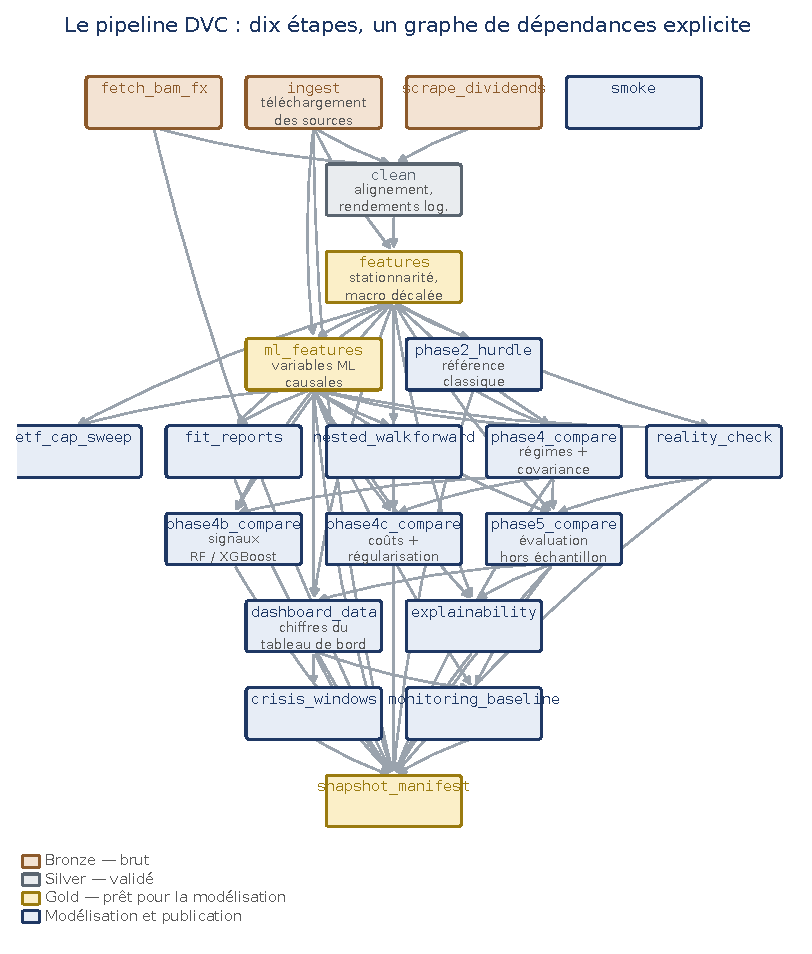
\includegraphics[width=0.92\textwidth]{assets/figures/pipeline_dvc.pdf}
  \caption[Le pipeline DVC]{Le pipeline de bout en bout~: dix étapes et
  vingt-et-une dépendances explicites, de la collecte des sources aux chiffres
  affichés par le tableau de bord. Cette figure est \emph{engendrée à partir du
  fichier de configuration du pipeline}~: elle ne peut pas décrire une chaîne
  différente de celle réellement exécutée.}
  \label{fig:pipeline}
\end{figure}

L'apport dépasse le confort. Le graphe rend le calcul \emph{invalidable}~: si une
donnée amont change, tous les résultats qui en dépendent sont marqués périmés,
qu'un humain s'en souvienne ou non. Le projet a appris cette leçon à ses dépens —
le fichier contenant la performance de référence à battre n'était initialement
pas suivi par le pipeline, et a dérivé d'une version de données sans que rien ne
le signale. Il est aujourd'hui une sortie d'étape à part entière.

\subsection{Dagster — « qu'est-ce qui doit se réexécuter, et quand ? »}

Dagster planifie l'exécution et matérialise la lignée
(figure~\ref{fig:dagster})~: neuf \emph{actifs} de données, chacun rattaché à sa
couche du médaillon, avec la date de leur dernière production. La règle imposée
au projet est que Dagster \emph{ordonnance} le traitement mais n'en contient
aucune logique~; ses actifs appellent les fonctions du code source, inchangées.

\begin{figure}[htbp]
  \centering
  \fbox{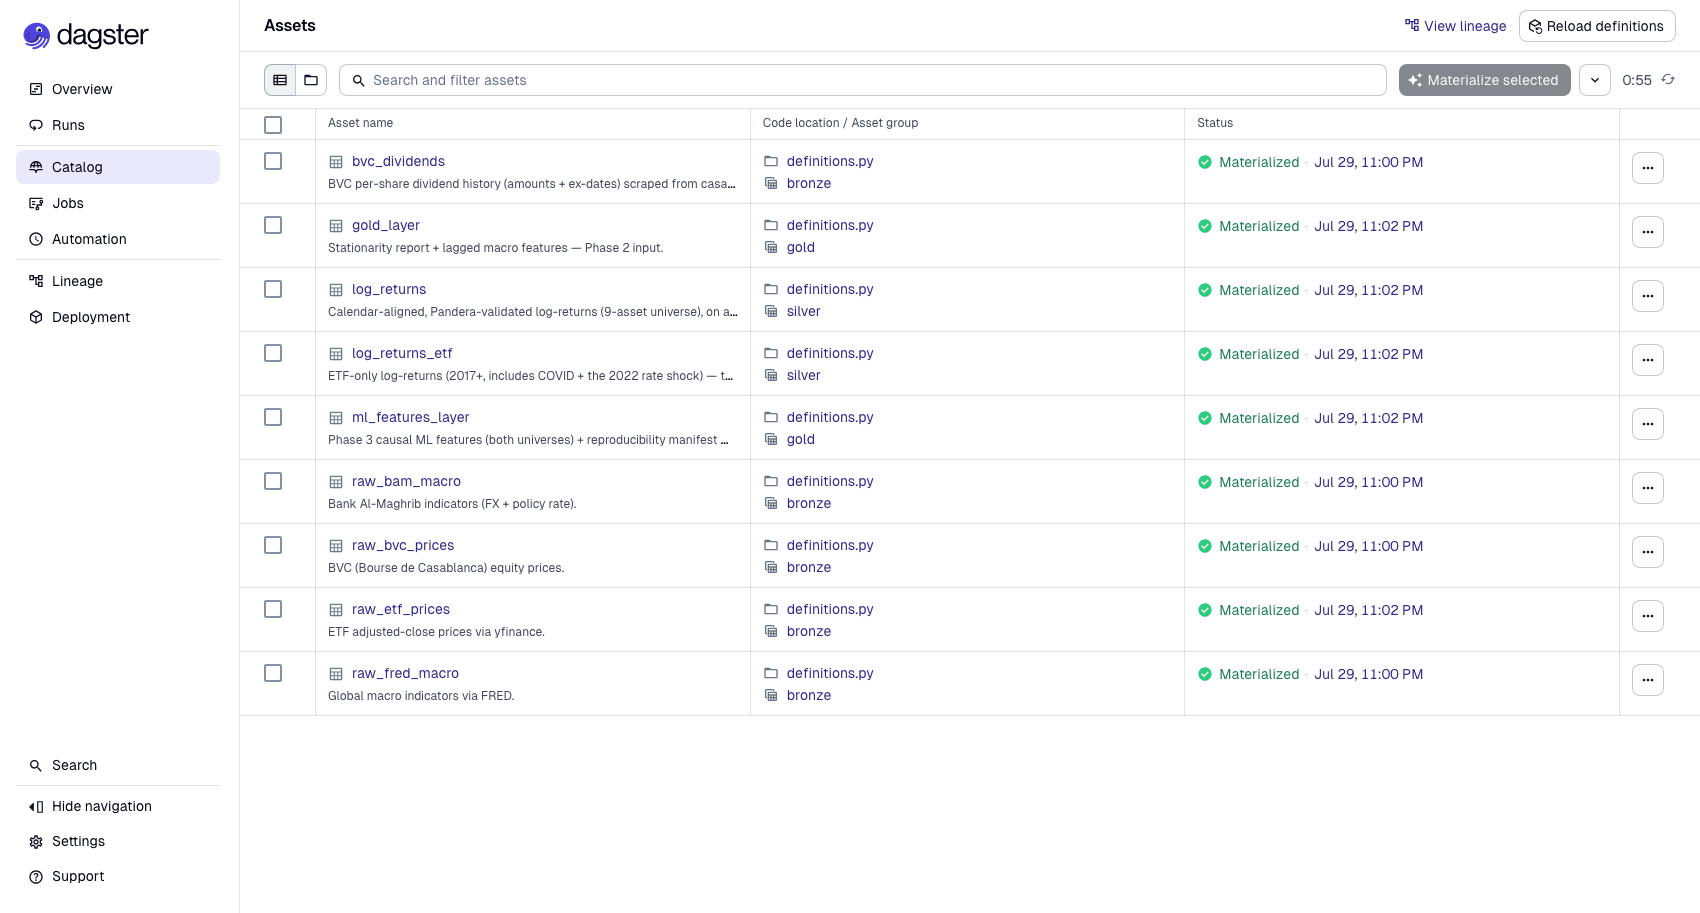
\includegraphics[width=0.95\textwidth]{assets/figures/dagster_assets.png}}
  \caption[Catalogue des actifs Dagster]{Catalogue Dagster~: les neuf actifs de
  données du projet, leur description, la couche à laquelle ils appartiennent
  (\texttt{bronze}, \texttt{silver}, \texttt{gold}) et l'état de leur dernière
  matérialisation. Toute sortie censée se rafraîchir automatiquement doit
  figurer ici — une omission a coûté au projet deux semaines de dérive
  silencieuse entre ses deux univers.}
  \label{fig:dagster}
\end{figure}

\subsection{MLflow — « d'où vient ce chiffre ? »}

MLflow enregistre les \emph{résultats}~: pour chaque exécution, les paramètres
employés, les métriques obtenues, le fichier source et le commit exact du code
(figure~\ref{fig:mlflow}). C'est le registre qui permet, six semaines après, de
répondre à la question « ce Sharpe de 1,164, sur quelles données et avec quels
réglages~? » sans relancer un calcul.

\begin{figure}[htbp]
  \centering
  \fbox{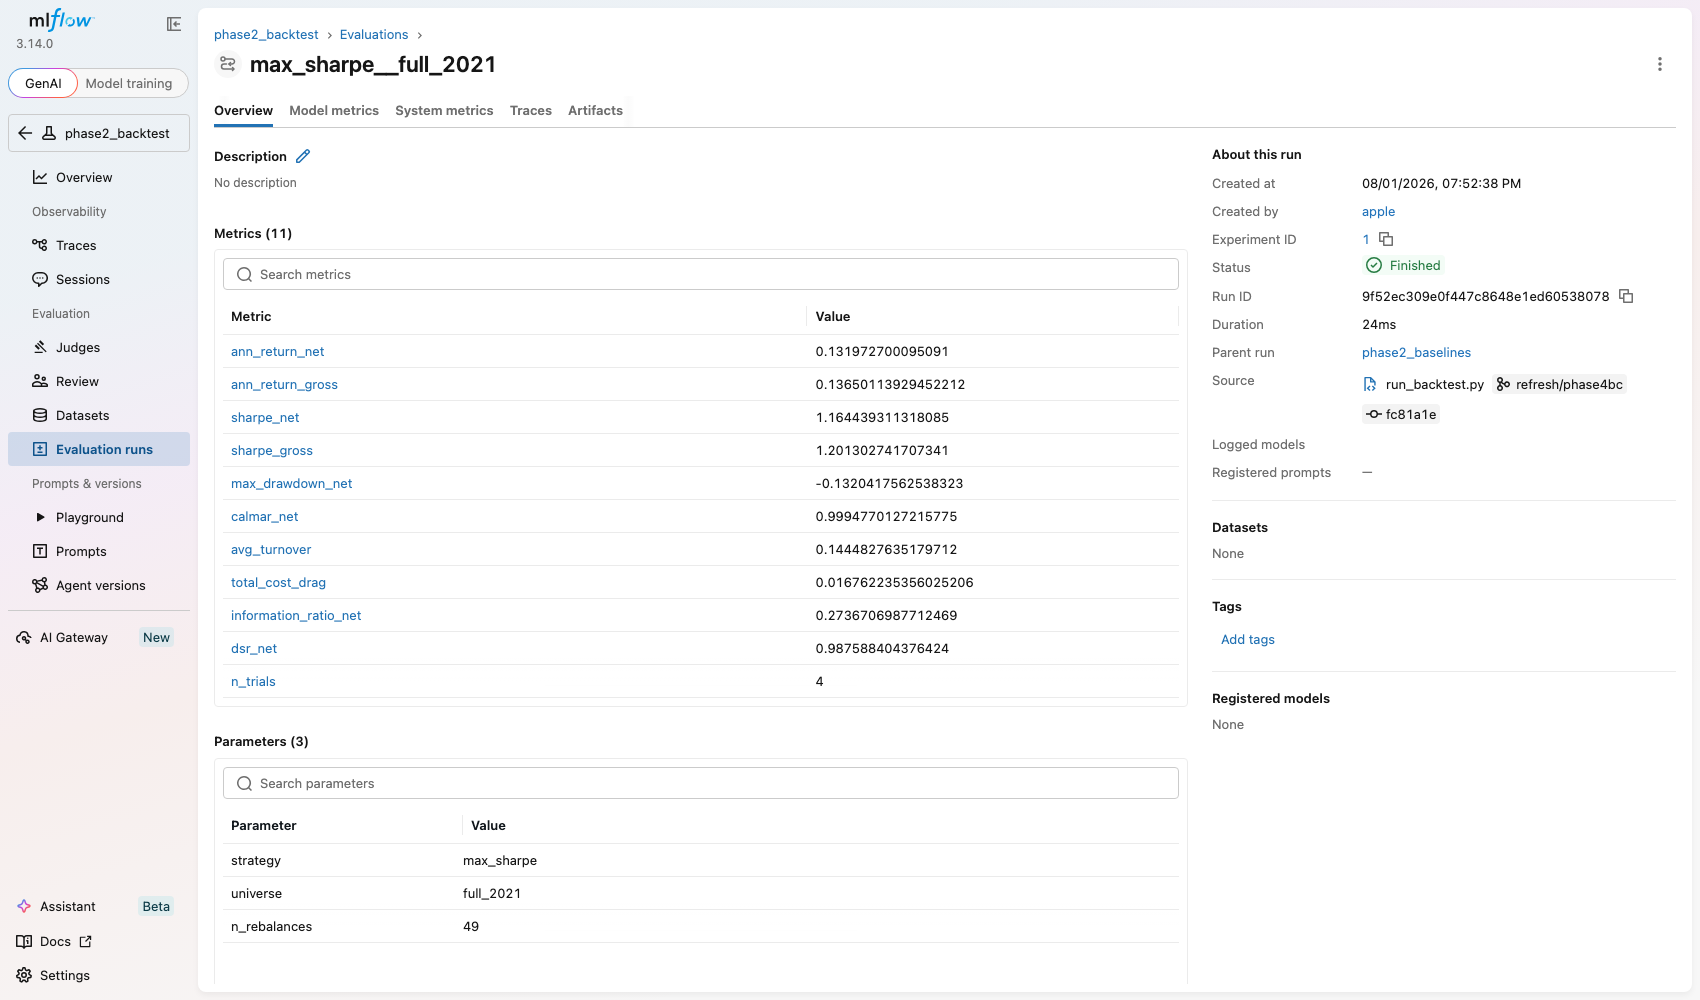
\includegraphics[width=0.95\textwidth]{assets/figures/mlflow_ui.png}}
  \caption[Suivi d'expérience MLflow]{MLflow~: détail d'une exécution. Les onze
  métriques enregistrées comprennent le ratio de Sharpe net (1,164 — la valeur de
  référence citée au chapitre~\ref{chap:resultats}), sa contrepartie brute, le
  drawdown, le turnover et le ratio de Sharpe déflaté. Le panneau de droite
  conserve le fichier lancé et le commit exact du code.}
  \label{fig:mlflow}
\end{figure}

\begin{remarquebox}
Ce registre a lui-même révélé un défaut lors de la préparation de ce chapitre~:
la version de MLflow employée n'écrivait \emph{que} les fichiers joints dans le
mode de stockage configuré, et abandonnait silencieusement paramètres et
métriques. L'interface affichait des exécutions vides. La configuration a été
corrigée et centralisée dans une fonction unique appelée par les six programmes
concernés — et la valeur de référence régénérée est identique au bit près à celle
publiée, ce qui confirme que seul l'enregistrement était en cause, non les
calculs.
\end{remarquebox}

% =============================================================================
\section{Ce que l'exploitation a appris}
% =============================================================================

Deux incidents méritent d'être rapportés, parce qu'ils ne relèvent ni de la
finance ni du ML, et que ce sont eux qui ont façonné les garde-fous décrits
plus haut.

\textbf{Un serveur de code périmé.} La tâche nocturne a échoué plusieurs jours de
suite sans que personne ne le sache. Le processus qui sert le code aux exécutions
planifiées avait démarré \emph{avant} la création d'un nouveau module~; il ne
pouvait pas l'importer, et rechargeait bien les définitions mais jamais l'état
d'importation de son interpréteur. Conséquence~: un univers se mettait à jour,
l'autre non — exactement la dérive que la double base de test rend visible. La
correction technique fut d'une ligne (importer le module au chargement plutôt
qu'à l'exécution, pour que la panne survienne immédiatement et bruyamment). La
vraie correction fut un test~: \emph{rien} dans la suite n'importait le paquet
d'ordonnancement, si bien que des centaines de tests passaient sur un pipeline
incapable de démarrer.

\textbf{Un artefact déchiré.} Une longue exécution de modélisation et
l'ordonnanceur nocturne partageaient le même répertoire de données. Le second a
reconstruit la couche Gold \emph{pendant} que la première la lisait~: le fichier
de résultats produit décrivait un univers avec des données au 24 juillet et
l'autre avec des données plus récentes. Aucune erreur, aucun avertissement — un
fichier parfaitement bien formé et faux. Les données ont été restaurées depuis le
cache de versionnement, l'ordonnanceur arrêté, l'exécution refaite avec une
assertion préalable sur la date des données. La leçon générale~: \textbf{une
exécution longue et un ordonnanceur actif ne doivent jamais partager un
répertoire de données}, et c'est ce cas précis que le test de cohérence entre
documents détecte désormais.

% =============================================================================
\section{La pile technique}
% =============================================================================

\begin{table}[htbp]
  \centering
  \small
  \caption[Pile technique]{Principaux outils et rôle de chacun.}
  \label{tab:pile}
  \begin{tabular}{@{}p{3.3cm}p{9.2cm}@{}}
    \toprule
    \textbf{Outil} & \textbf{Rôle dans le projet} \\
    \midrule
    Python, pandas, NumPy & Langage et calcul numérique. \\
    Parquet, DuckDB & Stockage en colonnes des trois couches~; requêtes
    analytiques sur la couche Gold. \\
    Pandera & Contrats de données appliqués à l'écriture (Silver et Gold). \\
    scikit-learn, SciPy & Rétrécissement de covariance de Ledoit-Wolf~;
    optimisation sous contrainte. \\
    \texttt{hmmlearn}, \texttt{arch} & Modèles de régime à états cachés~;
    modèles de volatilité. \\
    \texttt{xgboost} & Modèles de prédiction de rendement (chapitre~4). \\
    DVC & Versionnement des données et graphe de reproductibilité. \\
    Dagster & Ordonnancement local et lignée des actifs. \\
    MLflow & Journal des expériences~: paramètres, métriques, code. \\
    Streamlit, FastAPI & Tableau de bord à deux pages et interface REST. \\
    pytest & 390 tests, hors ligne, exécutés à chaque modification. \\
    \bottomrule
  \end{tabular}
\end{table}

Deux choix négatifs méritent d'être mentionnés, car ils ont été délibérés. Une
bibliothèque spécialisée de validation croisée pour la finance a été
\emph{écartée} au profit d'une implémentation interne d'une cinquantaine de
lignes, son modèle de licence étant devenu restrictif~: une dépendance dont
l'accès peut disparaître n'a pas sa place au cœur d'un dispositif d'évaluation.
Et aucun ordonnanceur d'entreprise n'a été retenu~: le projet s'exécute sur une
machine unique, et l'outil choisi cartographie directement les couches du
médaillon.

% =============================================================================
\section*{Synthèse du chapitre}
\addcontentsline{toc}{section}{Synthèse du chapitre}

\begin{itemize}
  \item Les données transitent par trois couches à sens unique, chacune validée à
        l'écriture~; la modélisation ne lit que la dernière.
  \item L'absence d'historique marocain avant 2021 est une limite assumée,
        compensée par une \textbf{double base de test} — toute stratégie est jugée
        sur deux univers, et les désaccords entre eux sont publiés.
  \item Le moteur de backtest, écrit une fois et jamais modifié, est une
        \textbf{frontière de confiance}~: il découpe les données que les modèles
        reçoivent et valide les décisions qu'ils rendent. L'impossibilité de voir
        le futur est un test, pas une convention.
  \item Les règles qui comptent sont exécutables~: hermétisme des tests,
        cohérence entre documents publiés, interdiction des chiffres écrits à la
        main, traçabilité P1--P4 (107~fonctions sur 110).
  \item DVC, Dagster et MLflow répondent à trois questions distinctes —
        \emph{ce résultat est-il à jour}, \emph{quand doit-il se recalculer},
        \emph{d'où vient ce chiffre}. Les trois incidents d'exploitation du projet
        ont chacun consisté en une réponse devenue fausse sans que rien ne le
        signale~; ils ont tous donné lieu à un garde-fou automatique.
\end{itemize}
